% Chapter Template

\chapter{Search Cloud} % Main chapter title

\label{Chapter6} % for referencing this chapter elsewhere, use \ref{ChapterX}

\lhead{Chapter 6. \emph{Search Cloud}} % this is for the header on each page - perhaps a shortened title
\section{Overview}
\texttt{SF1R} could be deployed as a fully distributed search engine. Within \texttt{iZENECloud}, we have it supporting different kinds of search requests, 
some of which require non-distributed deployment while others are deployed distributedly, as shown in figure \ref{fig:searchcloud}. We call such platform
as a search cloud.
\begin{figure}[!ht]\centering
  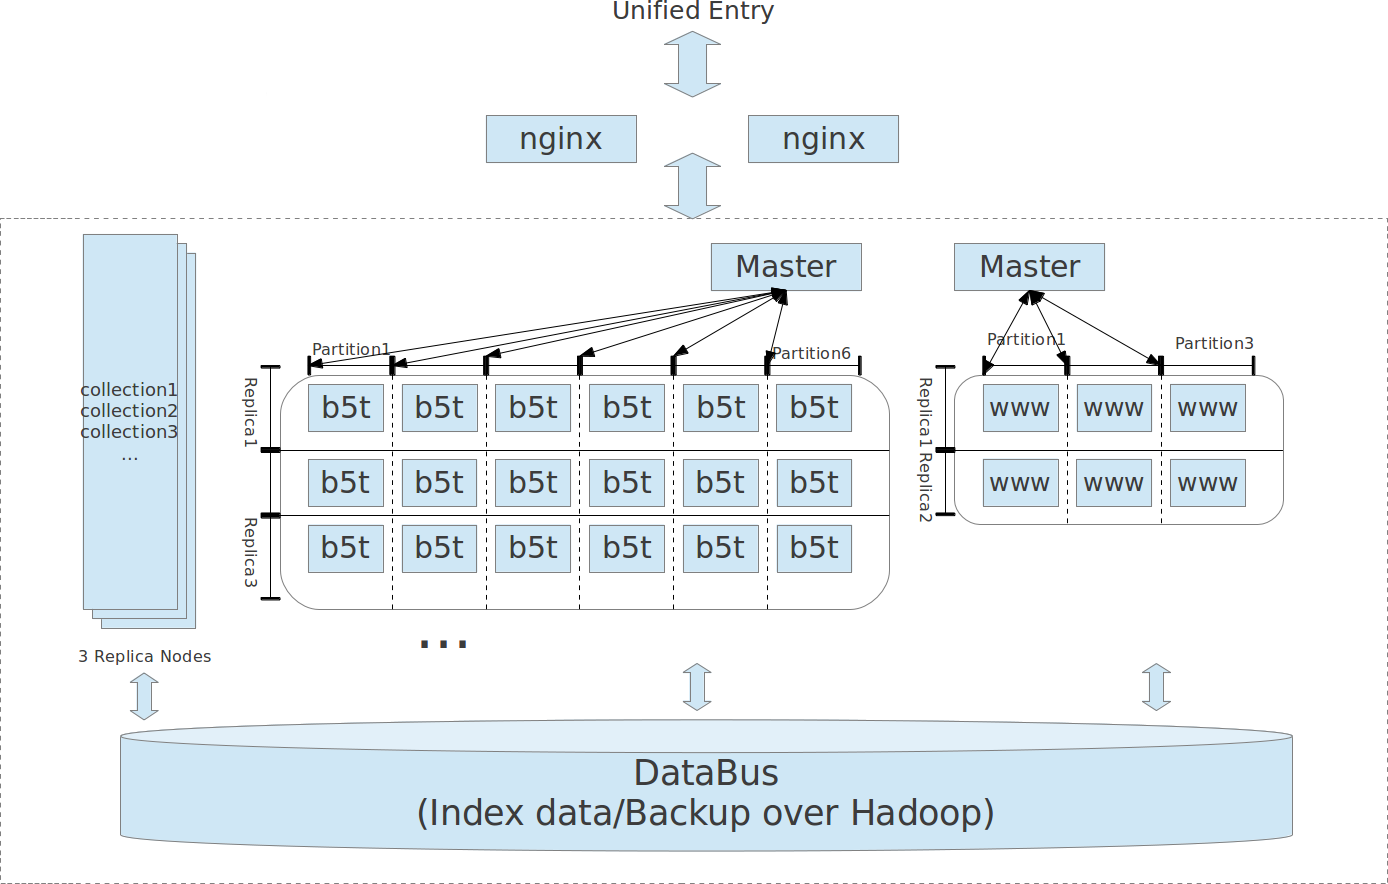
\includegraphics[width=.90\textwidth]{Figures/searchcloud.png}
  \caption{SF1R Search Cloud}\label{fig:searchcloud}
\end{figure}


The overview of \emph{Distributed SF1R} nodes is shown in \ref{fig:overview}. Each Node can have several replicas, and all the replicas in the same replica 
set have the same nodeid. We call them together as a replica set. Basically, there will be one primary node and some secondary nodes in the specific replica
set. Each node will supply the master and worker parts.

\begin{figure}[!ht]\centering
  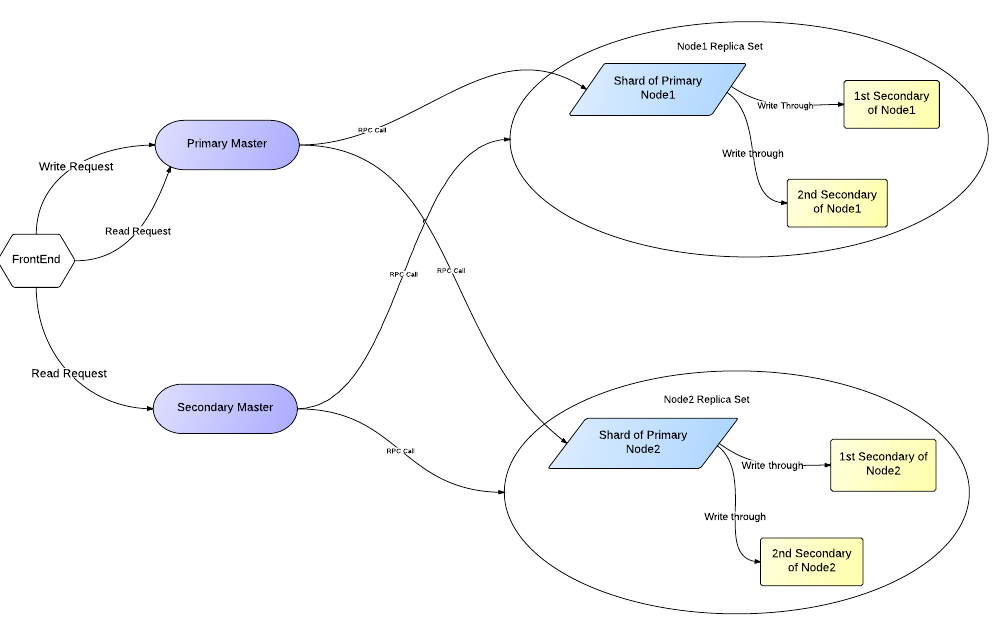
\includegraphics[width=.90\textwidth]{Figures/overview.png}
  \caption{Distributed SF1R Architecture}\label{fig:overview}
\end{figure}
\begin{figure}[!ht]\centering
  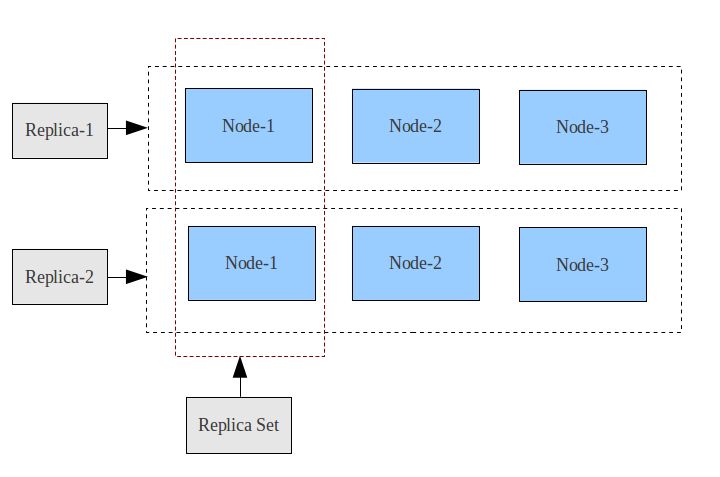
\includegraphics[width=.70\textwidth]{Figures/replica-set.png}
  \caption{Distributed SF1R Replica Set}\label{fig:replica-set}
\end{figure}

\begin{enumerate}
 \item \emph{Primary Master} \newline
   The master part on the primary node, it will take charge of distributing the search request to all shard workers and merging the results from all shard workers. And also take the charge of pulling the write request from zookeeper and distribute the write request to all shard workers on primary.

 \item \emph{Secondary Master} \newline
   The master part on the secondary node, it will take charge of distributing the search request to all shard workers and merging the results from all shard workers. And also take the charge of pushing the write request to zookeeper.
 \item \emph{Shard Worker} \newline
    The worker part on the node will do the actually work as one of shard worker and return the result to the master. For write request, the shard worker on primary node will take charge of broadcasting the request to all secondary nodes in the same replica set.
\end{enumerate}

\section{Architecture and Internal}
\subsection{The role of ZooKeeper}
    The ZooKeeper in the distributed sf1r will serve as the node activity detecting and primary electing. The distributed write queue is also used in the zookeeper to make sure all write request can be saved temporally. In sync mode, the zookeeper is used to keep the processing state of write request and notify the primary and the secondary nodes about the state changes. By using zookeeper we can make sure all nodes  will see the same topology view in the distributed sf1r since the zookeeper has implemented the PAXOS protocols to make sure the data consistency. The topology in zookeeper is as below:
\begin{lstlisting}
/                                  # Root of zookeeper namespace
|--- SF1R-[CLUSTERID]              # Root of distributed SF1 namesapce, 
                                   [CLUSTERID] is specified by user configuration.

      |--- Topology                # Topology of distributed service cluster
           |--- Replica1           # A replica of service cluster
                |--- Node1         # A SF1 node in the replica of cluster, it can be a 
                                     Master or Worker or both.
                |--- Node2
           |--- Replica2
                |--- Node1
                |--- Node2

      |--- Servers                 # Servers in topology is a master node.
           |--- Server00000000
                     |--- Search, Recommend       # A master node supply Search and 
                                                  #  Recommend service as master
           |--- Server00000001
      |--- WriteRquestQueue                       # Root of waiting write request queue
           |--- Node1                             # Waiting Write request queue for node1
                |--- WriteRequestSeq0000000000    # the waiting write request
           |--- Node2
      |--- PrimaryNodes
           |--- Node1                             # backup primary nodes for node1 
                |--- Primary0000000000            # first backup primary server as current                                                                
                                                  #  primary for replica set node1.
                |--- Primary0000000001            
           |--- Node2
                |--- Primary0000000000
                |--- Primary0000000001
      |--- WriteRequestPrepare                    # prepare root node for sync write
           |--- Node1                             # prepare for node1 in sync write.
           |--- Node2
      |--- Synchro                 # For synchronization task

\end{lstlisting} 
    
    
\subsection{The new write routine on distributed sf1r}

\begin{figure}[!ht]\centering
  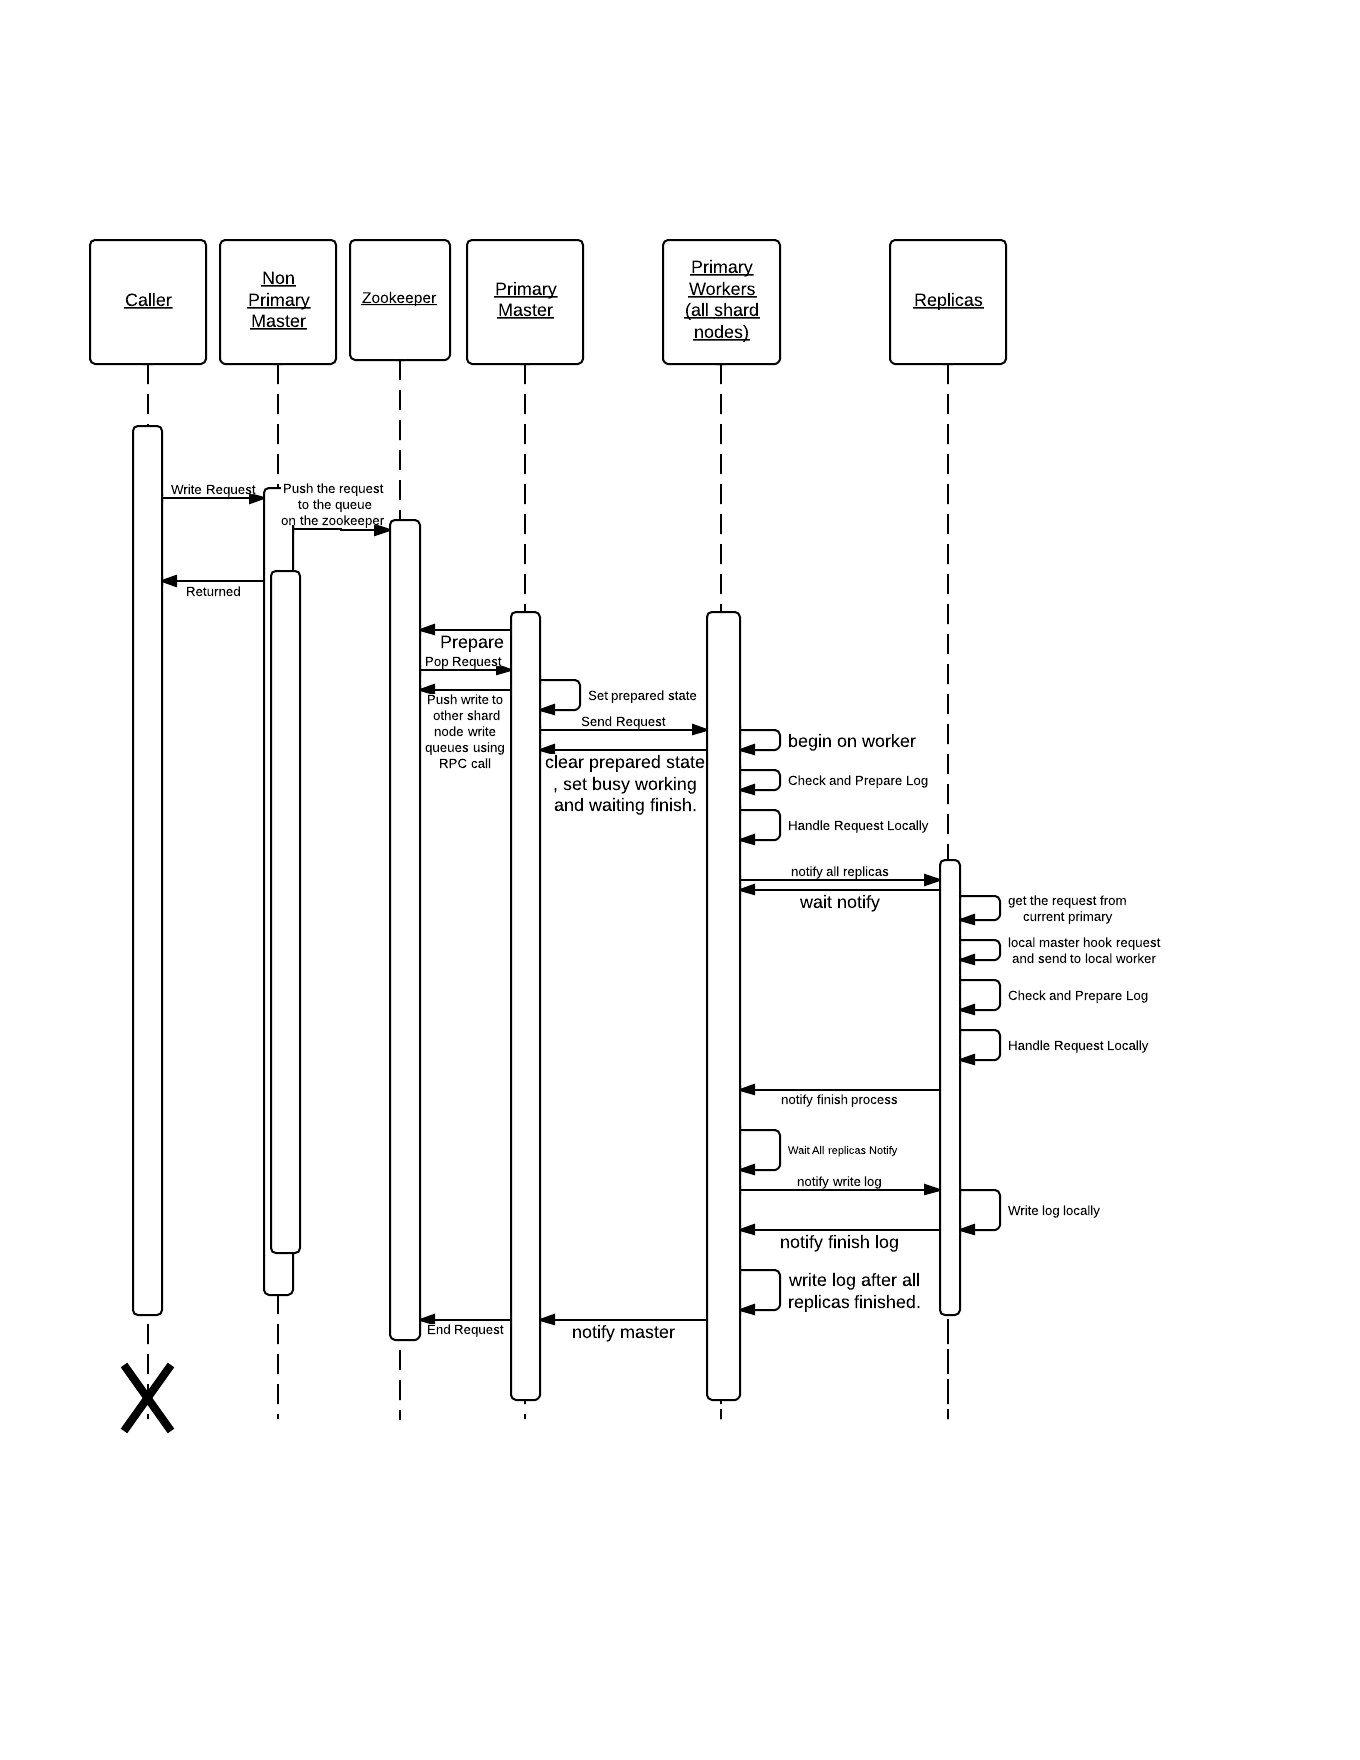
\includegraphics[width=.90\textwidth]{Figures/WriteRequestProcess.png}
  \caption{Write request handling Flow}\label{fig:writeprocess}
\end{figure}

Figure \ref{fig:writeprocess} has shown the working flow of the write request:
\begin{enumerate}
 \item A client caller send write request to one of node in the specific replica set on distributed sf1r.
 \item The master part on the node will push the request to the write queue on zookeeper. For each replica set it has a standalone write queue on the zookeeper for its own.
 \item The primary node will be notified and try to get the new write from zookeeper. If success, the master part on primary node will set the prepared state and pop the write request from the queue.
 \item If the write request should be distributed to other shard workers, it will be pushed to the write queue belong to that shard node.
 \item The primary shard worker begin process on local. After finished on primary worker, it will notify other nodes in the same replica set by updating the zookeeper nodedata. Then the primary worker will wait all secondary nodes until finished or down by accidentally.
 \item The secondary worker will be notified by zookeeper while there is a new write from primary. After the secondary worker finished, it will notify the primary by updating the zookeeper nodedata and wait the primary to get ready to write log.
 \item After all secondary finished the write request(or part of them down), the  primary will notify all secondary to write the log.
 \item The secondary worker will get notified from primary after all secondary finished write request. Then it will write the log to disk and notify primary that the log has been written.
 \item After all secondary finished writting log, the primary worker will write log to disk and the write request is finished finally.
 \item The primary worker notify the primary master on the same node that it is ready for next new request. And the primary master will check if any new request on the write queue and continue to handle the next write request.
\end{enumerate}

\subsection{Starting Node In Distributed SF1R}
How a node start in distributed sf1r is shown as below: \ref{fig:nodestart}. Starting a node will add a secondary to the replica set if there is already a primary, otherwise the starting node will enter the replica set as a primary.

\begin{figure}[!ht]\centering
  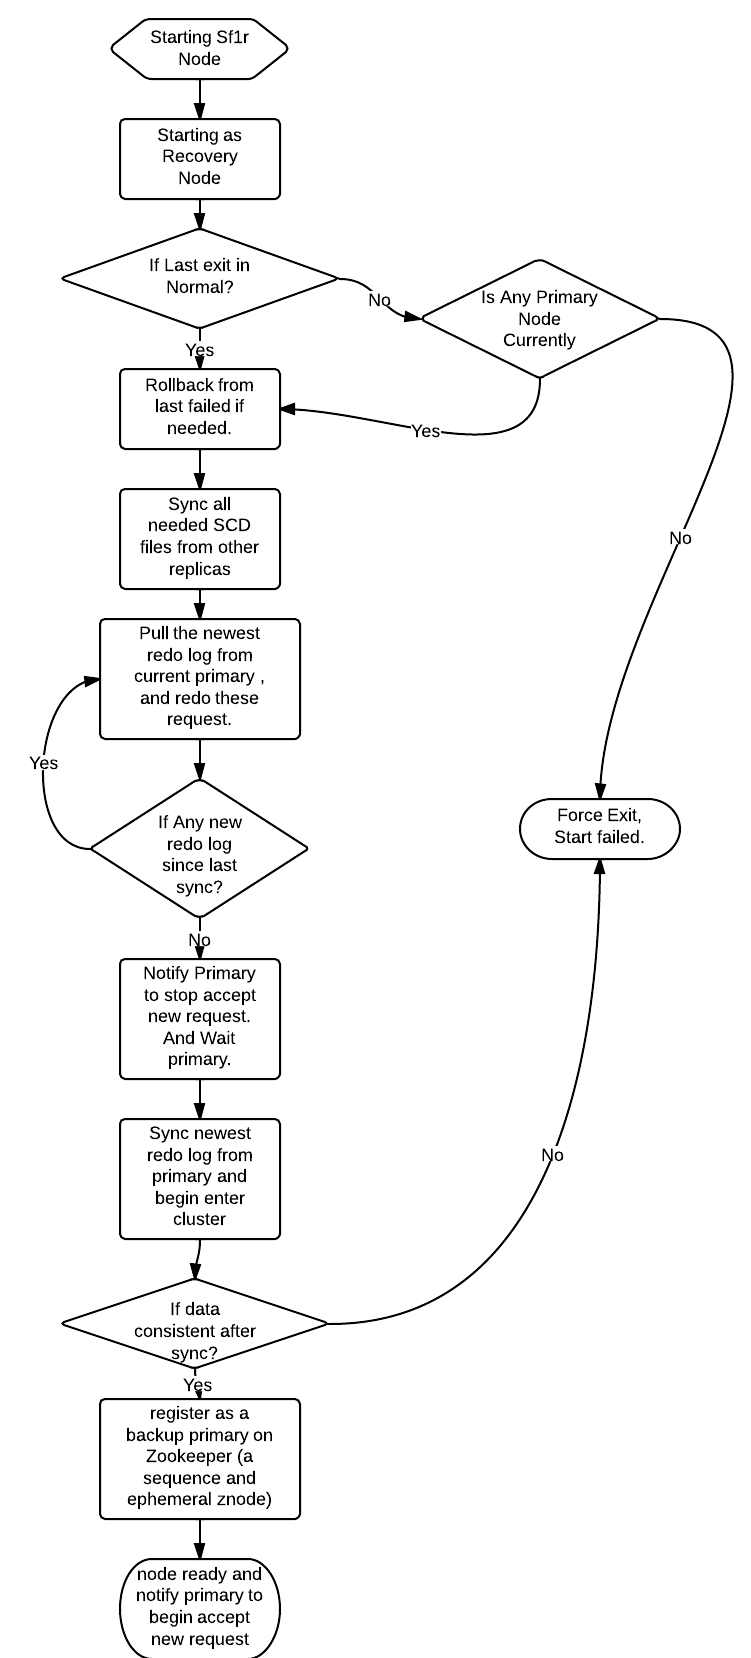
\includegraphics[width=.60\textwidth]{Figures/nodestart.png}
  \caption{Starting of a node}\label{fig:nodestart}
\end{figure}

\begin{enumerate}
 \item \emph{Staring node as primary}\newline
Each distributed node will be registered as a backup primary node in the same replica set on the zookeeper. The first backup primary node in the replica set will be treated as primary.

  \begin{itemize}
   \item Check data: while starting, the node will check whether local data is ok by checking if some flag file exists on local. If last down by accidentally, the node can not be started as primary. Because we can not identify the correctness of the local data without checking by comparing with the other node.
   \item Register as backup primary: After checking data, the first node will start and register a backup primary in the replica set. Because this is the first backup primary, it will be treated as the current primary. The start is finished at last.
  \end{itemize}

 \item \emph{Starting as secondary}\newline
After the first node in the replica set started, all other nodes will be started as secondary.

 \begin{itemize}
 \item Recover: If last exit is normal, no recovery needed. Otherwise, the secondary will restore the data from the newest backup.
 \item Sync to Newest log: After recovery finished, the secondary will pull new log data from primary, and redo the log since last down. After synced to the newest log, the secondary will notify the primary to stop accecpt new request and begin to enter cluster.
 \item Check consistent: If primary agreed the enter of secondary, the secondary will check the data consistent with primary by computing the CRC of the collection data files. If the consistent finished success the node starting as secondary is done at last. Otherwise, the secondary node will fail to start.
 \end{itemize}
 
\end{enumerate}

\subsection{Failing in Distributed SF1R}
In distributed sf1r, there are many cases to cause a failing node. Basically, there are two major fails: primary fail and non-primary fail. Beside, because the zookeeper is used, we need handle the zookeeper connection lost as one kind of fail. The handle of fail is shown in Fig \ref{fig:nodefail}.
\subsubsection{Abort write request}
If the write request failed to finished, the node need rollback to the state before write. This is aborting a write request.
\begin{itemize}
\item When abort hanppen: Abort may happen if the primary failed to finish or a secondary send abort request to primary. The expired session on zookeeper connection while running request will also trigger the aborting. 
\item How to abort: While aborting triggered, the primary node will notify all secondary nodes to abort the request. If the secondary node did not begin to run the write, the abort can ignore since no write happen on the node. Otherwise, the secondary node will do the aborting and notify primary after aborting finished. While aborting on the local node, it will find the latest backup and restore data from it. After that the node will redo the logs between the latest backup and current failed state. By redoing the log, the node can restore state to the old state before the failed write actually running.
\end{itemize}
\subsubsection{Auto failover and recover}
The master will be notified if the fail node is in the watching list of master and the master will try to failover this node by using the backup node with the same nodeid in other replica set. If the fail node restarts later, the master will recover this node.
\subsubsection{Primary Fail}
Current primary fail will trigger a backup primary to begin electing and the backup primary will take the charge of primary if its log is newest.
\begin{enumerate}

\item Primary fail while idle: While idle, the primary fail will notify all replicas in the same replica set and the first backup primary will become new primary and notify all other replicas by updating self state to electing. The other backup nodes will just update the current primary info and notify the new primary that I am ready to follow the new primary. After all other nodes followed the new primary, the new primary will end the electing and ready for the next new write request.
\item Primary fail while write request running local: If the primary failed while running the write request but not finished yet. Because the other nodes in the replica set haven't began to run the write, we can handle it just the same as case 1.
\item Primary fail While write request finished local: In this case, some of the secondary nodes have already begun to run write request on the node. So we need abort the current write request if the node has begun and after aborting the node will reenter the cluster to sync to the new primary. If the node has not yet start to run the write, it can begin electing the same as case 1.
\item Primary fail while ready to write log: In this case, all secondary nodes have already finished write request, but not all secondary nodes finished the log. This is almost the same as the case 3 except the node finished log do not need to abort the current write request. All others not finished log need abort request and re-enter cluster.
\item Primary fail while electing: In this case, it means the current primary failed and the first backup also failed while trying to become new primary. It is almost the same as the case 1 except the second backup take charge of the new primary.
\item Primary fail while others recovering: In this case, the recovering node need follow the new primary and redo recovering from the mew primary. The nodes not recovering can be handled just like the other case in 1-5.
\end{enumerate}

In all case above, the node re-enter cluster if the log is fall behind others. The newest log id will be updated to zookeeper once the node finished log.

\subsubsection{Non-Primary Fail}
\begin{enumerate}

\item Non-Primary fail while idle: Nothing will happen except auto failover on master since no write running.
\item Non-Primary fail while write request running local: The primary will stop waiting this fail node and check if others finished the write request.
\item Non-Primary fail while recovering: The primary will stop waiting this node to enter cluster and check if any new write request can be handled.
\item Non-Primary fail while electing: The new primary will stop waiting this node to follow itself and check if others followed it.

\end{enumerate}

\begin{figure}[!ht]\centering
  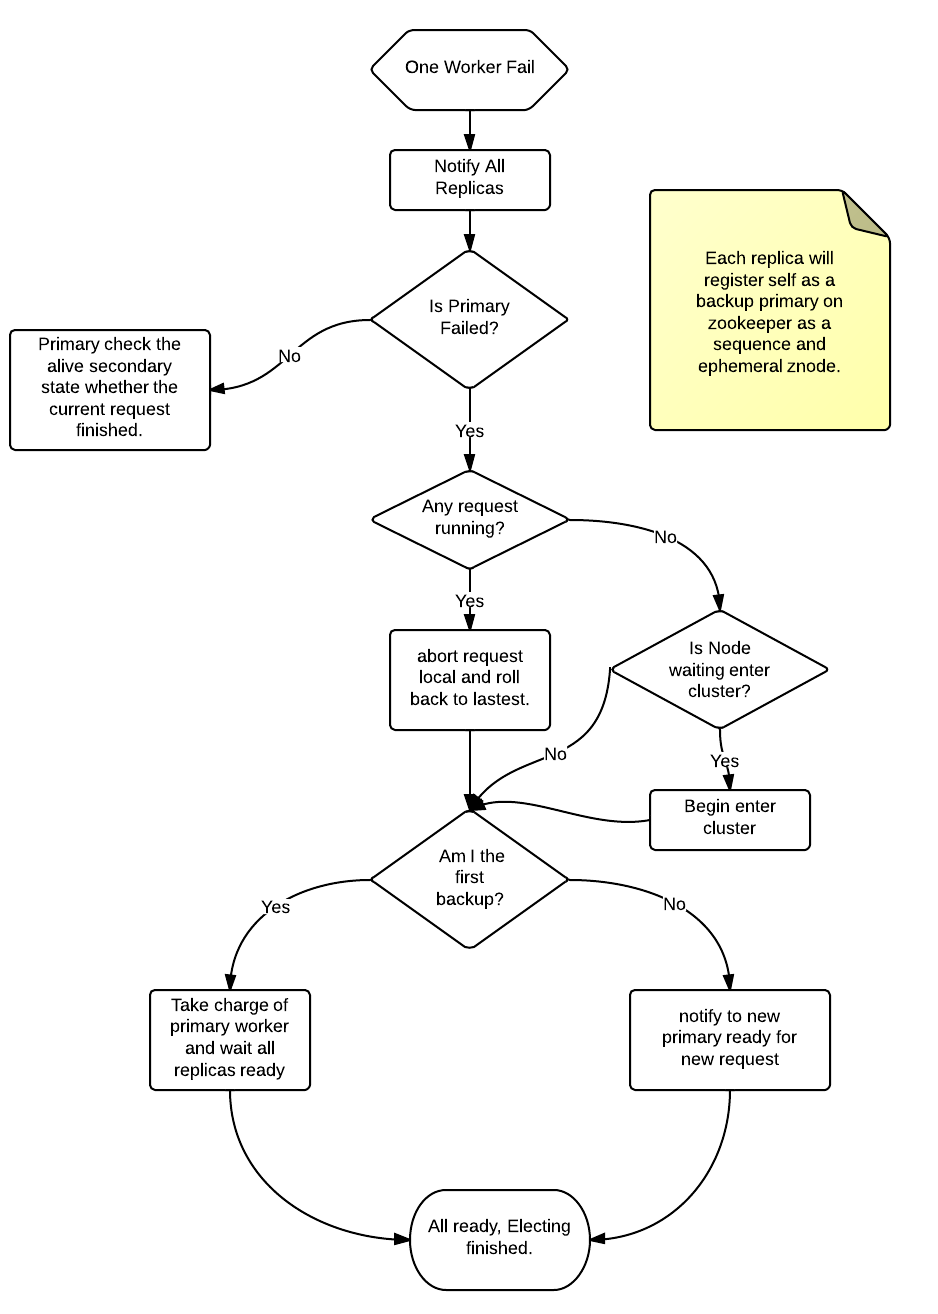
\includegraphics[width=.60\textwidth]{Figures/NodeFail.png}
  \caption{Fail of a node}\label{fig:nodefail}
\end{figure}

\subsubsection{ZooKeeper Connection Lost}
ZooKeeper will lost connection by auto-reconnect or expired session. This may happen while network is unstable or zookeeper server is restarting.
\begin{itemize}
\item Auto-reconnect: In this case, the zookeeper will make sure all nodes created by self keep the same after auto-reconnected. But we need refresh other nodes state such as primary or other secondary nodes after auto-reconnect finished. If primary node has changed during auto-reconnect, the node need do the same thing just like the primary fail case. If nothing happened during auto-reconnect, the node can continue to run without any change.
\item Expired Session: expired session will cause all zookeeper self-created node and event invalid, so we need reconnect to the zookeeper by hand. After expired, the node will set the state and keep waiting until the node is ready to re-enter cluster. Any unfinished write will be aborted.
\item Optimization for the unstable zookeeper: Sometimes the zookeeper is very unstable and we need do some optimization to avoid the unnecessary change of primary node and the abortion of the running write request. This can be done by checking the primary aliveness so we can make sure the electing only start when the primary is really unreachable. In this way, the temporally lost for the primary will not trigger the primary election or write abortion.  
\end{itemize}
 
\subsection{Async write support}
As described above, the write need keep communicating with zookeeper while doing the write. This will cause much downgrade of write performance if there are many replicas in the replica set because of the network latency. In order to improve the  performance of write, the async write has been implemented to reduce the communication with zookeeper while handling the write request. 
\begin{itemize}
\item Async write on primary node: On primary the write flow is almost the same as sync except the notify to zookeeper has been just ignored. In async write, the primary will pop the write request from zookeeper and handle it locally without notify others and keep going on until no more new write on zookeeper. As we can see, the communication with zookeeper has been reduced to only 1 time. This will greatly improve the write performance and will keep the same even the replica set become larger.
\item Async write on secondary node: Since the primary no long notify secondary about the write request, the secondary nodes will pull the redo logs from current primary periodically and redo these logs in the log sync thread. 
\item Drawback of async write: As we can see, the secondary nodes may fall behind from primary node, and if primary failed part of logs may have not synced to other secondary nodes. This will cause write request loss.
\item Recovering in async mode: Since the failed primary may have the logs that other secondary nodes don't have, while the failed primary restarting, the node need check whether the log is newer that current new primary. If restarting with newer log, the node need rollback to old and sync to new primary.

\end{itemize}

\subsection{SF1R lib for distributed SF1R}

\begin{figure}[!ht]\centering
  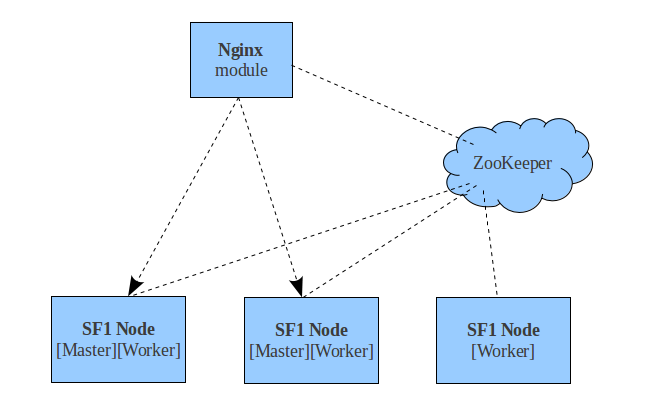
\includegraphics[width=.60\textwidth]{Figures/nginx-sf1rlib.png}
  \caption{The SF1R lib for nginx}\label{fig:sf1rlib}
\end{figure}

The SF1R lib in Fig \ref{fig:sf1rlib} is used by the distributed nginx. By using this sf1r-lib the client can send request with no need for knowing the topology in the distributed sf1r. This client lib will find the correct sf1r node in topology automatically and send the request to it. The client lib update the topology by using the zookeeper connection and any changes from zookeeper will be notified.
  
\begin{itemize}
\item Support For Separating read and write: Currently, the distributed sf1r node will write the current busy state to the zookeeper while the busy state changed. By reading the busy state from zookeeper node we can temporally disable the read from the node who is busy writing. In this way, we can route the read request and write request to different nodes to implement separating the read and write.
\end{itemize}

\subsection{The Sharding for the huge data}
While the data growing rapidly, the single node can not handle all the data anymore. Then we need do the sharding of the data to put the data across several nodes.
\begin{itemize}
\item Benefit: improve read/write performance.
 Concurrently read and write on different nodes is more effective than multi-thread r/w on the single node because there is no CPU contention.
\item What to think: The first thing is load balancing, we should make sure all sharding nodes are handling the average work. The second thing is to handle the add/remove sharding nodes easily since the data may grow rapidly.
\item How to do: Using consistent hashing to keep data balance among all sharding nodes and avoid too much data migrate while changing the sharding nodes topology. Pick up the searching worker one by one to balance the read request among them.
\end{itemize} 


\section{Developer Guide}
Because all the write request will be handled on primary first and send to all secondary nodes from primary, the new write request need some adjustment to be adopted by distributed sf1r. Most work has been done and we can add new write simply follow as below step:

\subsection{Add new write api}

\begin{enumerate}

\item add the controller+action string in the function initWriteRequestSet in the RequestLog.cpp file.
\item if the write api is in the controller that derived from Sf1Controller, then most work will be done OK in base class. If not, you need handle it yourself.
\item If the api will execute on all shard workers, you need push the write request to the queues of other shard workers. (See the index write request in the class IndexTaskService for example.)
\item In the write request handler, coding as below:
\begin{lstlisting}[language=C]
// check valid first.
DISTRIBUTE_WRITE_BEGIN;
DISTRIBUTE_WRITE_CHECK_VALID_RETURN;
// do pre-check without modify any collection data. 
if (precheckfailed())
{
    return false;
}

// prepare request log before actually modify the collection data.
CreateOrUpdateDocReqLog reqlog;
reqlog.timestamp = Utilities::createTimeStamp();
if(!distributereqhooker->prepare(ReqCreateOrUpdate_Doc, reqlog))
{
    LOG(ERROR) << "prepare failed in " << __FUNCTION__;
    return false;
}

// do modify collection data.
ret = modify_data();
if (!ret)
{
    return false;
}
// flush data to make sure data write to disk.
flush();

DISTRIBUTE_WRITE_FINISH(ret, reqlog);
return ret;
\end{lstlisting}
\item Make sure the controller and handler will execute in sync.
\item If an api will call another write api, you should set the chain status properly.
\item Define a new req log type in RequestLog.h if necessary and set for rollback and backup action in DistributeRequestHooker.cpp file.

\end{enumerate}

\subsection{Add new write cron job}
In order to run cron job in distributed mode, the cron job need a job name cronJobName for each cron job and each cron job just do one job. cronJob task is a function with calltype parameter. You should write cron job function as below:
\begin{lstlisting}[language=C]
void RecommendTaskService::cronJob_(int calltype)
{
    if (cronExpression.matchesnow() || calltype > 0)
    {
        // check if need to put the job to distributed sf1r write queue.
        if(calltype == 0 && NodeManagerBase::get()->isDistributed())
        {
            if (NodeManagerBase::get()->isPrimary())
            {
                MasterManagerBase::get()->pushWriteReq(cronJobName_, "cron");
                LOG(INFO) << "push cron job to queue on primary : " << cronJobName_;
            }
            else
                LOG(INFO) << "cron job ignored on replica: " << cronJobName_;
            return;
        }
        // check for valid
        DISTRIBUTE_WRITE_BEGIN;
        DISTRIBUTE_WRITE_CHECK_VALID_RETURN;
        // prepare the log for cron job.
        CronJobReqLog reqlog;
        reqlog.cron_time = Utilities::createTimeStamp();
        if (!DistributeRequestHooker::get()->prepare(Req_CronJob, reqlog))
        {
            LOG(ERROR) << "!!!! failed running cron job. : " << cronJobName_ << std::endl;
            return;
        }
        //do the job task here. and flush data after job finished. 
        bool ret = DoJob();
        flush();
        //finish job
        DISTRIBUTE_WRITE_FINISH(ret);
    }
}
\end{lstlisting}

\subsection{Add new write callback}
The write callback is used for the write without any write api or cronJob. You can add/remove a write callback with an identify string and call it as below :

\begin{lstlisting}[language=C]

// add new callback.
DistributeDriver::get()->addCallbackWriteHandler(collection_ + "_callBackFuncName",
    boost::bind(&CallbackObj::callbackFunc, this, _1));

// removing the callback
DistributeDriver::get()->removeCallbackWriteHandler(collection_ + "_callBackFuncName");

// call callback by push the specific data.
DistributeDriver::get()->pushCallbackWrite(reqloghead.req_json_data, reqdata);

\end{lstlisting}

The callbackFunc should have the protocol as below and should be with the log type ReqCallback:
\begin{lstlisting}[language=C]
bool callbackFunc(int calltype);
\end{lstlisting}

The calltype will be used to tell who is calling this callback. In the callback you should code just like the write request api handler.

\subsection{Auto test}
Currently, the distributed sf1r support auto test for new write request. The auto test will try all possible fail case to check if data is consistent after the write request.

For each write request api, you can add the test json request body to the autotest directory. All the json file under it will be tested in all kinds of node fails to make sure after the write request we  get the consistent data.

If you want some node fail at the some test point, you can do
\begin{lstlisting}[language=C]
echo failtype > distribute_test.conf 
\end{lstlisting}
under the working directory. the \emph{failtype}  here stand for the kind of test point at which line the sf1r will fail. Currently all test points are shown as below:
\begin{lstlisting}[language=C]
enum TestFailType
{
    NoAnyTest = 0,
    NoFail,
    PrimaryFail_At_Electing,
    PrimaryFail_At_BeginReqProcess,
    PrimaryFail_At_PrepareFinished,
    PrimaryFail_At_ReqProcessing,
    PrimaryFail_At_NotifyMasterReadyForNew,
    PrimaryFail_At_AbortReq,
    PrimaryFail_At_FinishReqLocal,
    PrimaryFail_At_Wait_Replica_Abort,
    PrimaryFail_At_Wait_Replica_FinishReq,
    PrimaryFail_At_Wait_Replica_FinishReqLog,
    PrimaryFail_At_Wait_Replica_Recovery,
    PrimaryFail_At_Master_PrepareWrite,
    PrimaryFail_At_Master_checkForNewWrite,

    ReplicaFail_Begin = 30,
    ReplicaFail_At_Electing,
    ReplicaFail_At_Recovering,
    ReplicaFail_At_BeginReqProcess,
    ReplicaFail_At_PrepareFinished,
    ReplicaFail_At_ReqProcessing,
    ReplicaFail_At_Waiting_Primary,
    ReplicaFail_At_Waiting_Primary_Abort,
    ReplicaFail_At_AbortReq,
    ReplicaFail_At_FinishReqLocal,
    ReplicaFail_At_UnpackPrimaryReq,
    ReplicaFail_At_Waiting_Recovery,

    OtherFail_Begin = 60,
    Fail_At_AfterEnterCluster,
    Fail_At_CopyRemove_File,

    FalseReturn_Test_Begin = 70,
    FalseReturn_At_UnPack,
    FalseReturn_At_LocalFinished,
};

\end{lstlisting}

\section{Operation Note}
\subsection{Configuration}
A simple sample configuration is as below:

SF1R Node1, work as Master and Shard Worker 1. For this Master, it provides multiple collections, "b5mp" is distributed to two shard workers.

part of sf1config.xml
\begin{lstlisting}
    <DistributedTopology enable="y">
      <CurrentSf1rNode nodeid="1" replicaid="1">
        <!--master names for B5M are www|stage|beta-->
        <MasterServer enable="y" name="undefined" />
        <WorkerServer enable="y" />
      </CurrentSf1rNode>
    </DistributedTopology>
\end{lstlisting}

part of b5mp.xml
\begin{lstlisting}
    <IndexBundle>
      <ShardSchema>
        <ShardKey name="DOCID" />
        <DistributedService type="search" shardids="1,2" />
        <DistributedService type="recommend" shardids="1,2" />
      </ShardSchema>
      ...
    </IndexBundle>
\end{lstlisting}

SF1R Node2, work as Master and Shard Worker2 (with shard 2).
\begin{lstlisting}
    <DistributedTopology enable="y">
      <CurrentSf1rNode nodeid="2" replicaid="1">
        <MasterServer enable="y" name="undefined" />
        <WorkerServer enable="y" />
      </CurrentSf1rNode>
    </DistributedTopology>
\end{lstlisting}

The \emph{name} in Master Server can be used to tell the difference for independent cluster such as the beta/stage/www cluser.

\subsection{Monitor status}
Some node status will be updated to memory statistical data. If you want to get the running status of distributed sf1r node, you can using the api
\begin{lstlisting}
status/get_distribute_status
\end{lstlisting}
From this we can known the current primary host and how many write request processed and etc..

\subsection{Update SF1R}
The update can have two major cases: simple update and update to new cluster. The simple update will happen while the update is compatible with old node, otherwise update to new cluster is needed.
\begin{itemize}
\item Update config: replace the config file on current primary node and send the api command
\begin{lstlisting}
collection/update_collection_conf 
\end{lstlisting}
After this the updated config will auto deliver to other replicas in the replica set.
\item Simple update: If the data or code is compatible with the old one, we can do simple update. Just using the script below:
\begin{lstlisting}
distribute_tools.sh simple_update new-sf1r-tar-file
\end{lstlisting}
and wait until the updating node can serve as the new master or worker.

\item Update to new cluster: update to new cluster is needed while the new is no longer compatible with the old. We can do this one by one as follow : 
\begin{enumerate}

\item Chose one node in the replica set and run the script :
\begin{lstlisting}
distribute_tools.sh update_to_newcluster new-sf1r-tar-file new-clusterid
\end{lstlisting}
\item Rebuild data if needed by using the api.
\item Backup node data. Using api
\begin{lstlisting}
collection/backup_all
\end{lstlisting}
to generate the backup data on the current node.
\item Copy the backup data to other replicas and update the left nodes one by one. On the other nodes, using the script 
\begin{lstlisting}
distribute_tools.sh rollback new-clusterid
\end{lstlisting}
to restore the data from the copied backup data. After all nodes have finished, the update to new cluster is done.

\end{enumerate}
\end{itemize}
\subsection{Handle Unexpected down}
The node in distributed sf1r may be down at any time. After started, the node will set a force exit flag file and this flag file will be removed if the node is stopped normally. While starting, if the force exit flag exists, we treat it as an accident down. In this case we will restore the data from the latest backup and sync to newest from current primary.

While running the write request, the node will set a rollback flag file to indicate the current running request with the request id. If the write failed to finish, we can know which state we will rollback to. If the rollback file is empty it will rollback to the latest backup.

If all nodes in the replica set are down, we need check the log data carefully. We need find out which node has the newest log data and start this node as the first node in the replica set.
